\documentclass[12pt,a4paper]{report}
\usepackage[utf8]{inputenc}
\usepackage[a4paper,
            left=2.5cm,
            right=2.5cm,
            top=2.5cm,
            bottom=2.5cm]{geometry}
\usepackage{appendix} 
\usepackage{graphicx,amsmath}
\graphicspath{{images/}}
\usepackage{titlesec}
\usepackage{wrapfig}
\usepackage{enumitem}
\usepackage[backend=biber,style=authoryear]{biblatex}
\addbibresource{references.bib}
\usepackage{hyperref}
\usepackage{booktabs}
\usepackage[T1]{fontenc}
\usepackage{lmodern}
\usepackage{textcomp}
\hypersetup{pdfborder={0 0 0}}

\setlist[itemize]{%
  itemsep=0.1em,
  topsep=0.1em,
  parsep=0pt,
  partopsep=0pt
}

\setlength{\parindent}{0pt}
\setlength{\parskip}{0.3em}

\titleformat{\chapter}[hang]
  {\normalfont\Large\bfseries}
  {\thechapter.}
  {1em}
  {}
\titlespacing*{\chapter}{0pt}{2em}{0.2em}

\titleformat{\section}[block]
  {\normalfont\large\bfseries}
  {\thesection\ }
  {1em}
  {}
\titlespacing*{\section}{0pt}{0.5em}{0.5em}

\title{
  \vspace{-2em}
  
\includegraphics[width=4cm]{luiss.png}\\[1.5em]
  {\LARGE Finance and Financial Technologies}\\[0.5em]
  {\large Group Project: Oracle \& Pirelli}
}
\author{Alice Alessandrelli \and Yassir El Arrag \and Matilde Tambini \and Shefik Memedi \and Leonardo Farfan Rodriguez}
\date{Group 3\\April 2025}

\usepackage{etoolbox}
\makeatletter
% Remove the \clearpage that report.cls inserts before every \chapter
\patchcmd{\chapter}{\clearpage}{}{}{}
\makeatother


\begin{document}

\maketitle
\pagenumbering{gobble}
\tableofcontents
\clearpage

\pagenumbering{arabic}
\setcounter{page}{1}

\chapter{Introduction}
\noindent
\begin{minipage}[t]{0.65\textwidth}
\section*{Oracle Corporation}
NYSE: ORCL \textbar\ Austin, Texas, USA
\end{minipage}%
\hfill
\begin{minipage}[t]{0.30\textwidth}
  \vspace{-12pt}
  
\includegraphics[width=\linewidth]{oracle.png}
\end{minipage}\\

\textbf{CEO:} Safra A. Catz \\
\textbf{Chairman \& Co-Founder:} Larry Ellison

\textbf{Industry:} Enterprise Software and Cloud Computing

Oracle, founded in 1977, is a global leader in enterprise software, hardware and cloud (OCI) services--spanning database management and ERP--for finance, healthcare, retail and telecom. In FY 2024 it generated \$53 billion in revenue (+6\% YoY), including \$39.4 billion from cloud services (+12\%).\\

\textbf{Recent Developments:} In early 2025, Oracle announced a \$500 billion AI infrastructure partnership with OpenAI and SoftBank called Stargate. The company is also deepening its multi-cloud strategy through new partnerships with Google Cloud and NVIDIA, reflecting its commitment to next-gen enterprise tech.\\

\noindent
\begin{minipage}[t]{0.65\textwidth}
\section*{Pirelli \& C. S.p.A.}
BIT: PIRC \textbar\ Milan, Italy
\end{minipage}%
\hfill
\begin{minipage}[t]{0.30\textwidth}
  \vspace{-12pt}
  
\includegraphics[width=\linewidth]{pirelli.png}
\end{minipage}\\

\textbf{CEO:} Andrea Casaluci (since 2023)\\
\textbf{Chairman:}  Jiao Jian \textbar\ \textbf{Executive Vice Chairman:} Marco Tronchetti Provera (previous CEO)

\textbf{Industry:} Automotive - High-End Tire Manufacturing

Founded in 1872, Pirelli is a globally recognized manufacturer of high-end tires for cars, motorcycles, and bicycles. Known for innovation and motorsport engagement, it operates in over 160 countries with 18 production facilities. In FY 2024, Pirelli reported preliminary revenues of approximately ~\texteuro6.9B, driven by high-value and EV tire demand.

\textbf{Recent Developments:}  In 2024, Pirelli faced governance tensions between Italian and Chinese shareholders, postponing its financial report and suspending U.S. investments due to regulatory concerns.  The company is however considering significant investments in the U.S. to mitigate potential impacts from possible tariffs, aiming to increase production capacity and maintain its market position. Pirelli also recently launched its fifth-generation P Zero tyre, using AI and virtual testing, and was named the exclusive tire supplier for all MotoGP categories starting in 2027.\\


\chapter{Valuation Framework}
\section{Comparable Company Analysis}
We began by examining each company's diluted EPS over the past five years and benchmarking against key industry peers. Oracle demonstrated steady, mostly uninterrupted earnings growth--underscoring both resilient profitability and strong investor confidence--while Pirelli's earnings climbed until 2023 before flattening, reflecting its more cyclical nature. Fair values were then estimated using both P/E and P/B multiples (based on five-year average EPS), with Oracle trading at a premium to peers such as Microsoft and IBM, suggesting the market is pricing in continued innovation-driven expansion. In contrast, Pirelli's more modest multiples versus Bridgestone and Continental imply either a value opportunity or market anticipation of slower growth.

To adjust valuation for growth, we calculated year-on-year rates for revenue, net income, total assets, and EPS. Oracle consistently delivered double-digit growth--led by AI infrastructure and cloud services--alongside widening operating margins. Pirelli, however, saw more moderate top-line gains, flatter margins, and a slight net-income decline by 2024. Incorporating these trends into the PEG ratio yielded approximately 1.67 for Oracle--highlighting a premium valuation relative to its growth trajectory--while Pirelli's negative PEG (due to expected earnings contraction) points toward a defensive, income-oriented profile.

\section{Intrinsic Valuation}
\textbf{Discounted Cash Flow (DFC) Valuation}

Using a forward-looking DCF model, we forecasted free cash flows (FCFs) for each company from 2024 through 2028, then calculated a terminal value with a 2.5\% perpetual growth rate. Oracle's projected FCFs were discounted at its WACC of 7.49\%, producing an enterprise value which, when divided by 2.85 billion outstanding shares, yields an intrinsic share price. A parallel methodology for Pirelli--assuming 5\% annual FCF growth through 2028 and discounting at a 7.5\% WACC--resulted in a per-share value based on its 1.06 billion shares. These DCF valuations underscore Oracle's premium growth potential versus Pirelli's steady, value-oriented cash generation.\\

\textbf{Dividend Policy \& Dividend Discount Model (DDM) Valuation}

From 2020 to 2024, Oracle raised its dividend per share from \$1.04 to \$1.60, with payout ratios between 28\% and 56\%--yet the yield fell from 1.72\% to 0.96\% due to strong stock appreciation. Applying a Gordon-growth DDM (g = 2.5\%, r = 8\%) yields an intrinsic value of \$29.82, well below the \$129.76 market price. Pirelli's annual dividends showed a high 272\% payout in 2020 before stabilizing at 41-53\%, producing yields above 3.5\%. Using g = 2\% and r = 10\% in the DDM gives a fair value of \$2.72 versus a \$5.76 share price. These results indicate dividends alone provide limited insight into Oracle's stock, while Pirelli's higher yield reflects its income-focused, value-stock character.

\section{Fixed-Income Valuation}
To complement equity analysis, we selected one bond from each issuer and applied standard discounting techniques--using yield to maturity (YTM), duration, and benchmark spreads--to estimate fair bond prices. Oracle's fixed-coupon bond traded slightly below par, consistent with its BBB credit rating and stable investor expectations. Pirelli's floating-rate issue, by contrast, traded above par, reflecting its shorter maturity and inflation-protected structure, which appeal to cautious investors. When mapped against recent market trends, both bonds' pricing patterns aligned with broader macroeconomic sentiment and issuer-specific risk profiles.

\chapter{Capital Structure \& Cost of Capital}
\section{Capital Mix}
Oracle's balance sheet is characterized by a strong equity base: as of FY 2024, it reported \$106.7 billion in market equity against \$41.8 billion of interest-bearing debt, resulting in capital structure of approximately 72\% equity and 28\%debt. This conservative leverage profile underpins its ability to fund large, innovation-driven investments without over-reliance on borrowed funds.

By contrast, Pirelli exhibits a more balanced capital mix, reflective of its steady industrial-manufacturing cash flows. While precise book values are not disclosed in our summary, the firm's combination of equity and debt financing aligns with its mid-cycle operations and provides a moderate cushion against market cyclicality.

\section{Cost of Equity (CAPM)}
We estimated each company's cost of equity via the Capital Asset Pricing Model:
\begin{itemize}
\item \textbf{Oracle}: Assumed inputs were a 4.0\% risk-free rate, a 5.5\% equity risk premium, and a beta of 1.0. Plugging into CAPM ($R_e=R_f+\beta(R_m-R_f)$) yields a cost of equity of 9.5\%.
\item \textbf{Pirelli}: Employed the same 4.0\% risk-free rate and 5.5\% market premium, but substituted a higher beta--reflecting its greater sensitivity to global economic swings. This adjustment produces a correspondingly higher cost of equity, consistent with its more cyclically exposed business model.
\end{itemize}

\section{Cost of Debt (after-tax)}
Oracle's after-tax cost of debt was calculated by dividing its annual interest expense by total debt and then applying a 21\% corporate tax shield, resulting in an effective borrowing rate of approximately 2.4\%. Pirelli's debt cost similarly reflects its actual interest burdens on total liabilities, net of corporate taxes; while the specific rate is not disclosed here, its use of both fixed--and floating-rate instruments--coupled with tax deductibility--yields a comparably modest after-tax cost of debt.

\section{WACC}
Combining these components, Oracle's WACC stands at 7.49\%, a rate that balances its strong equity cushion with affordable debt financing and supports long-term, innovation-focused investments. Pirelli's WACC is marginally higher at 7.5\%, reflecting its slightly elevated equity cost and balanced leverage, yet remains consistent with its steady, cyclical operations in the premium-tire market.

\chapter{Performance \& Market Diagnostics}
\section{Return on Equity (ROE)}
Annual ROE highlights each firm's ability to generate profit from shareholder equity. Oracle's ROE figures are exceptionally volatile, reaching 231.1\% in 2021, spiking to 544.9\% in 2023, and then moderating to 113.3\% in 2024. These extreme values primarily reflect aggressive share-buyback programs that drove book equity extremely low, making ROE a measure of both capital efficiency and financial engineering. Pirelli, by contrast, shows a much steadier ROE profile: climbing from single-digit percentages into the mid-teens before stabilizing, underscoring its more conservative capital structure and cyclically driven earnings.
\section{Beta Analysis}
We computed five-year betas using daily stock returns against two benchmarks per company using the standard beta formula (see Equation \ref{eq:beta}) Oracle's beta versus the NASDAQ Composite and NASDAQ-100 both sit around 0.70-0.72\, indicating its stock moves with the market but with less volatility than typical tech names. This lower-than-1.0 beta reflects Oracle's recurring-revenue model, which cushions it against abrupt market swings. Conversely, Pirelli exhibits higher systematic risk: its beta versus the FTSE MIB is approximately 1.08 (8\% more volatile) and versus the STOXX Europe 600 around 1.27 (27\% more volatile). As a cyclically sensitive industrial manufacturer, Pirelli offers higher return potential at the cost of greater share-price swings.
\section{Market Price vs. Computed Fair Price}
Comparing each share's market quote to our fair-value ranges derived from sector P/E and P/B multiples uncovers valuation gaps. Oracle's market price exceeds both multiples-based estimates, suggesting investors pay a premium for its robust growth prospects and innovative roadmap. Pirelli's share price, however, sits within or slightly below its computed fair range, indicating that the market may be pricing in modest growth or cyclical headwinds--and potentially offering a value entry point for patient investors.


\chapter{Portfolio Analysis}
In this section,  we examine the historical stock performance of Oracle Corporation and Pirelli \& C. S.p.A. over the past five years to construct optimal investment portfolios under the constraint of no short selling. The goal is to understand the trade-off between return and risk, identify optimal portfolios such as the minimum variance and maximum Sharpe ratio portfolios, and evaluate the benefit of diversification between these two assets. For this analysis, we used historical daily price data to calculate daily returns (see Equation \ref{eq:daily-return}).

The expected daily return for each stock was then estimated as the mean of its respective daily returns. Oracle showed an average daily return of approximately 0.1\%, while Pirelli had a lower expected daily return of about 0.047\%. Risk, defined as the standard deviation of daily returns, was similar for both stocks, approximately 2.2\%. To evaluate portfolio performance, we computed the covariance matrix of the returns, which captures both individual stock variances and their covariances. For a given portfolio with weights w, the expected return is given by the dot product in Equation \ref{eq:expected-return}, and the portfolio variance is computed with the Equation \ref{eq:portfolio-variance}.

Taking the square root yields the portfolio's standard deviation (volatility), which serves as a measure of risk. The feasible region of possible portfolios is constructed by varying the weight assigned to Oracle from 0 to 1. For each weight $w_{oracle}$ the corresponding weight of Pirelli is 1 - $w_{oracle}$. For every portfolio along this set, we computed the expected return, risk, and the Sharpe ratio (see Equation \ref{eq:sharpe-ratio}).

It was calculated assuming a daily risk-free rate of 0.02/252. For the efficient frontier, which represents the set of optimal portfolios that offer the highest expected return for a given level of risk, we computed the weights analytically using the solution derived from the Lagrangian optimization method. This involved solving the constrained optimization problem (see Equation \ref{eq:constrained-optimization-problem}).

The resulting weights were calculated for a range of expected portfolio returns $\mu_p$ between 0.0004 and 0.001, which covers the realistic bounds of achievable daily returns with these two assets. Since we worked under the assumption of long-only positions and weights summing to 1, the efficient frontier appears to closely resemble the feasible region (see Figure \ref{fig:appendix-feasible-region} and Figure \ref{fig:appendix-efficient-frontier}). However, they are fundamentally different: while the feasible region includes all possible portfolios formed by varying the weights between Oracle and Pirelli, the efficient frontier includes only the portfolios that maximize return for a given level of risk (or equivalently, minimize risk for a given return). In other words, for each level of risk, the efficient frontier contains only one optimal portfolio, making it a subset of the feasible region.

From the results of the efficient frontier, we observed that the Minimum Variance Portfolio (MVP) lies at the point with the lowest risk among all possible portfolios. It achieves an expected daily return of approximately 0.07\% with a risk (standard deviation) of 1.735\%. This portfolio allocates about 51\% of the investment to Oracle and 49\% to Pirelli. While its return is lower than that of the Maximum Sharpe Ratio Portfolio (MSRP), the significantly reduced volatility makes it appealing to risk-averse investors. In contrast, the MSRP delivers the best trade-off between return and risk, offering an expected return of 0.09\% with a risk of 1.936\%. This portfolio heavily favors Oracle, assigning it a weight of 82.1\%, while only 17.9\% is allocated to Pirelli. This allocation reflects Oracle’s higher average daily return (0.1\%) and slightly lower volatility compared to Pirelli (2.201\% versus 2.237\%). Interestingly, the MSRP is very similar to the portfolio in which we fully invest in Oracle, supporting the notion that Oracle is the more efficient asset on a risk-adjusted basis. On the other hand, fully investing in Pirelli resulted in the least attractive portfolio, with the lowest expected return (0.047\%) and highest volatility (2.237\%) among the options. This makes it the least desirable choice from a risk-return perspective (see Table \ref{tab:portfolio-results}).

In conclusion, this analysis illustrates how historical return and risk measures can guide portfolio construction and optimization. Depending on the investor's risk preference, different points on the efficient frontier provide rational choices: from the minimum variance portfolio for safety, to the maximum Sharpe ratio for optimized performance, to the high-return high-risk choice of full investment in Oracle. 



\chapter{Conclusions}
Across our multi-method analysis, Oracle and Pirelli emerge as clear representatives of growth and value investment styles, respectively.  

Oracle’s premium valuation parameters--P/E of 34.97 and P/B of 39.60--reflect lofty market expectations for continued innovation, while its low dividend yield of 0.96\% signals a reinvestment focus.  Its WACC of 7.49\% underpins a DCF-derived intrinsic value of \$76.73 per share, comfortably below today’s market price, validating its status as a growth-stock leader.  

By contrast, Pirelli exhibits hallmark value-stock features: a modest P/E of 11.76 and P/B of 0.97 suggest potential underpricing, while a robust dividend yield of 3.52\% caters to income investors.  Discounting its forecast cash flows at a 7.5\% WACC yields a fair value of \$12.02 per share--remarkably close to its market quote--confirming its defensive, value-orientation.  

Performance metrics reinforce these classifications.  Oracle’s ROE volatility--with peaks above 500\% driven by equity-reducing buybacks--underscores aggressive capital management, whereas Pirelli’s steadier ROE growth into the mid-teens highlights conservative financial stewardship.  Similarly, Oracle’s sub-1.0 betas versus the NASDAQ indices ($\approx$0.70-0.72) contrast with Pirelli’s higher cyclicality betas ($>$1.0 versus European benchmarks), mapping neatly onto their growth and value profiles.  

Finally, optimal portfolio construction demonstrates how these two stocks can be combined for tailored risk-return outcomes.  The minimum‐variance portfolio ($\approx$51\% Oracle, 49\% Pirelli) achieves a 0.07\% daily return at 1.735\% volatility, while the maximum‐Sharpe portfolio ($\approx$82\% Oracle, 18\% Pirelli) boosts return to 0.09\% at 1.936\% volatility--highlighting Oracle’s risk-adjusted efficiency alongside Pirelli’s stabilizing benefits.  

In sum, investors seeking capital appreciation and growth exposure will find Oracle’s profile most compelling, while those prioritizing income and cyclicality-hedged stability may favor Pirelli.  Blending both assets allows customization along the efficient frontier, aligning portfolio construction with individual risk-tolerance and return objectives.

\newpage
\appendix
\chapter{Additional Figures}
\begin{figure}[!htbp]
  \centering
  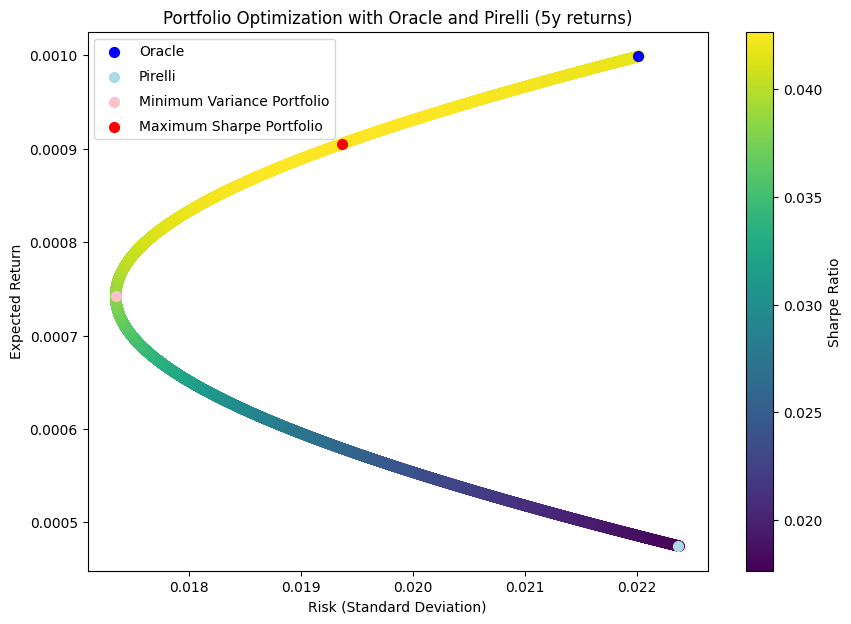
\includegraphics[width=0.8\textwidth]{feasible-region.png}
  \caption{Feasible Region of Portfolios (using Oracle and Pirelli).}
  \label{fig:appendix-feasible-region}
\end{figure}

\begin{figure}[!htbp]
  \centering
  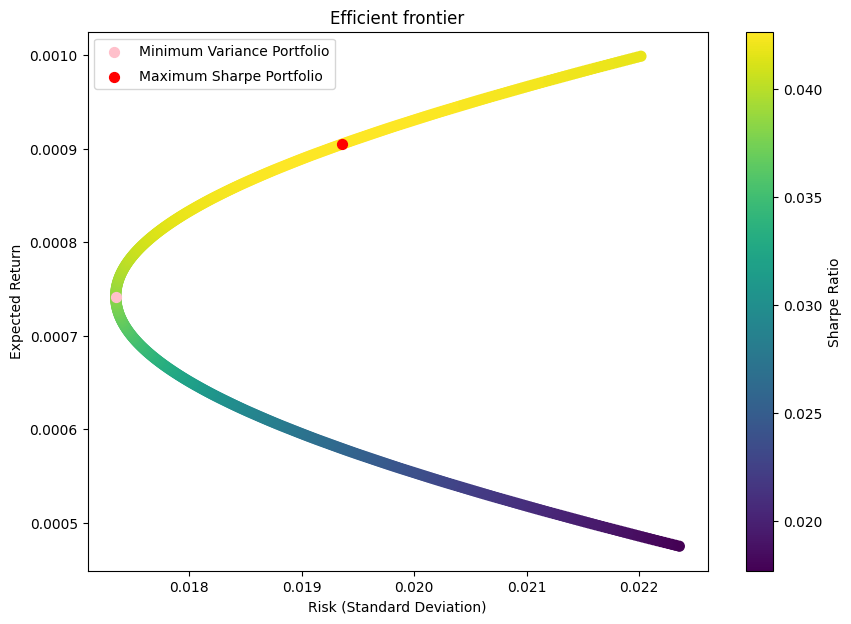
\includegraphics[width=0.8\textwidth]{efficient-frontier.png}
  \caption{Efficient Frontier.}
  \label{fig:appendix-efficient-frontier}
\end{figure}

\chapter{Tables}
\begin{table}[htbp]
  \centering
  \caption{Beta values for Oracle and Pirelli against computed with their markets}
  \label{tab:betas}
  \begin{tabular*}{\textwidth}{@{\extracolsep{\fill}} l l l l}
    \toprule
    Index/Portfolio & Covariance & Variance & Beta \\
    \midrule
    ORCL/\verb|^|IXIC & 0.00015819636 & 0.00021937652 & 0.72111803047 \\
    ORCL/\verb|^|NDX & 0.00016095824 & 0.00022841130 & 0.70468596766 \\
    PIRC/FTSEMIB.MI & 0.0001635459 & 0.0001518843 & 1.0767792396 \\
    PIRC/\verb|^|STOXX & 0.0001194998& 0.0000937962 & 1.2740366879 \\
    \bottomrule
  \end{tabular*}
\end{table}

\begin{table}[htbp]
  \centering
  \caption{Portfolios' results (using 5 years of historical data)}
  \label{tab:portfolio-results}
  \begin{tabular*}{\textwidth}{@{\extracolsep{\fill}} l l l l l}
    \toprule
    & Oracle & Pirelli & MVP & MSRP \\
    \midrule
    Return & 0.1\% & 0.05\% & 0.07\% & 0.09\% \\
    Risk & 2.20\% & 2.24\% & 1.70\% & 1.90\% \\
    Weights & [1, 0] & [0, 1] & [0.51, 0.49] & [0.821, 0.179] \\
    \bottomrule
  \end{tabular*}
\end{table}

\chapter{Formulas}
\begin{equation}
	\label{eq:beta}
	\beta=\frac{Cov(\Delta R_{stock}, \Delta R_{index})}{Var(\Delta R_{index})}
\end{equation}

\begin{equation}
	\label{eq:daily-return}
	r_t=\frac{P_t-P_{t-1}}{P_{t-1}}
\end{equation}

\begin{equation}
	\label{eq:expected-return}
	\mu_p=w\cdot\mu
\end{equation}

\begin{equation}
	\label{eq:portfolio-variance}
	\sigma_{p} = \sqrt{w^\top \Sigma w} = \sqrt{w_{ORCL}^2 \sigma_{ORCL}^2 + w_{PIRC}^2 \sigma_{PIRC}^2 + 2 w_{ORCL} w_{PIRC}Cov(ORCL, PIRC)}
\end{equation}

\begin{equation}
	\label{eq:sharpe-ratio}
	\text{Sharpe Ratio} = \frac{\mu_{p} - \mu_{f}}{\sigma_{p}}
\end{equation}

\begin{equation}
	\label{eq:constrained-optimization-problem}
	\begin{aligned}& \min_{w} \quad && w^\top \Sigma w \\ & \text{subject to} \quad && w^\top 1 = 1 \\ & && w ^\top \mu = \mu_{p} \end{aligned}
\end{equation}

\clearpage
\nocite{*}
\printbibliography

\end{document}
